\chapter{Laboratory 02b: solution}
\begin{QandAbox}
In order to solve this problem, \textit{SparsePOP} and \textit{Sedumi}, toolboxes should be installed, there exist one tutorial file.
\end{QandAbox}
consider the following problem:
\[
\begin{array}{c}
x^* = \arg\,\min\limits_{x} x_1^2 + x_2^2 - 4x_1 - 6x_2 + 13\\
\text{ s.t. }\\[1em]
x_1x_2 - 7x_2 = 10\\ [1em]
x_2 \geq -\frac{1}{2}x_1 +1
\end{array}
\]
The cost function here is a polynomial, which is a sum of \textit{monomial} terms. Each monomial is of the following form:
\[
\alpha x_1^{C_1} x_2^{C_2} \cdots x_n^{C_n}
\]

\begin{example}[Drawing the contour]
\begin{lstlisting}
clear; close all; clc;

%% Part 1: plot
x1_lw = -15; x1_up = +15;
x2_lw = -12; x2_up = +12;

x1 = linspace(x1_lw, x1_up);
x2 = linspace(x2_lw, x2_up);
% objective function
[X1,X2] = meshgrid(x1,x2);
Z = X1.^2 + X2.^2 - 4.*X1 - 6.*X2 + 13;
figure, contour(X1,X2,Z,5*(1:50)');

% equality constraint
x2_1 = linspace(0.01, x2_up);
x2_2 = linspace(x2_lw, -0.01);
x1_1 = (10+7.*x2_1)./x2_1;
x1_2 = (10+7.*x2_2)./x2_2;
hold on; plot(x1_1,x2_1, 'k',x1_2,x2_2, 'k');
axis([x1_lw,x1_up,x2_lw,x2_up]);
\end{lstlisting}
\end{example}


\begin{example}
\begin{lstlisting}
% inequality constraint
x2_ineq = -0.5*x1 + 1;
hold on; plot(x1, x2_ineq, 'b');
patch([x1(1); x1(end); x1_up; x1_lw], ...
    [x2_ineq(1); x2_ineq(end); x2_up; x2_up], ...
    'blue', 'FaceColor', 'blue', 'FaceAlpha', 0.1);
\end{lstlisting}
\end{example}
The resultant graph is as follows:

\begin{figure}[htbp]  % "h" for here, "t" for top, "b" for bottom, "p" for float page
    \centering
    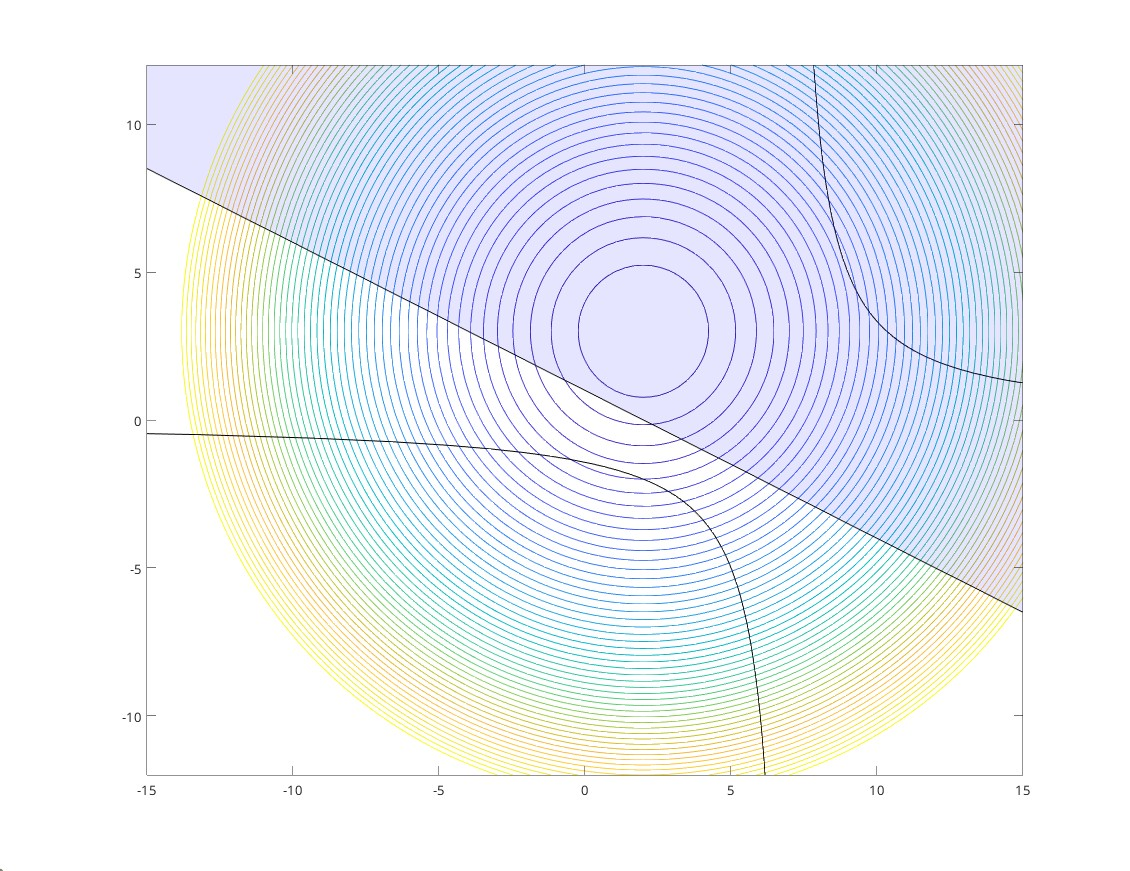
\includegraphics[width=0.75\textwidth]{images/lab02_contour.jpg}
    \caption{The contour of the polynomial as well as the graph of the constraints}
    \label{fig:constraints}
\end{figure}

Let's create the polynomial to be minized, named \textbf{objPoly}:

\begin{example}[Definig the polynomila to be optimized]
\begin{lstlisting}
% objective function
objPoly.noTerms = 5;
objPoly.dimVar = 2;
objPoly.typeCone = 1;  %always to be set to 1
objPoly.degree = 2; %the degree of the poly
objPoly.supports = [2 0; 0 2; 1 0; 0 1; 0 0];
objPoly.coef = [1, 1, -4, -6, 13]'; %should be a column vector
\end{lstlisting}
\end{example}
Pay attention that the support matrix should be made according to the following scheme:

\begin{figure}[ht]  % "h" for here, "t" for top, "b" for bottom, "p" for float page
    \centering
    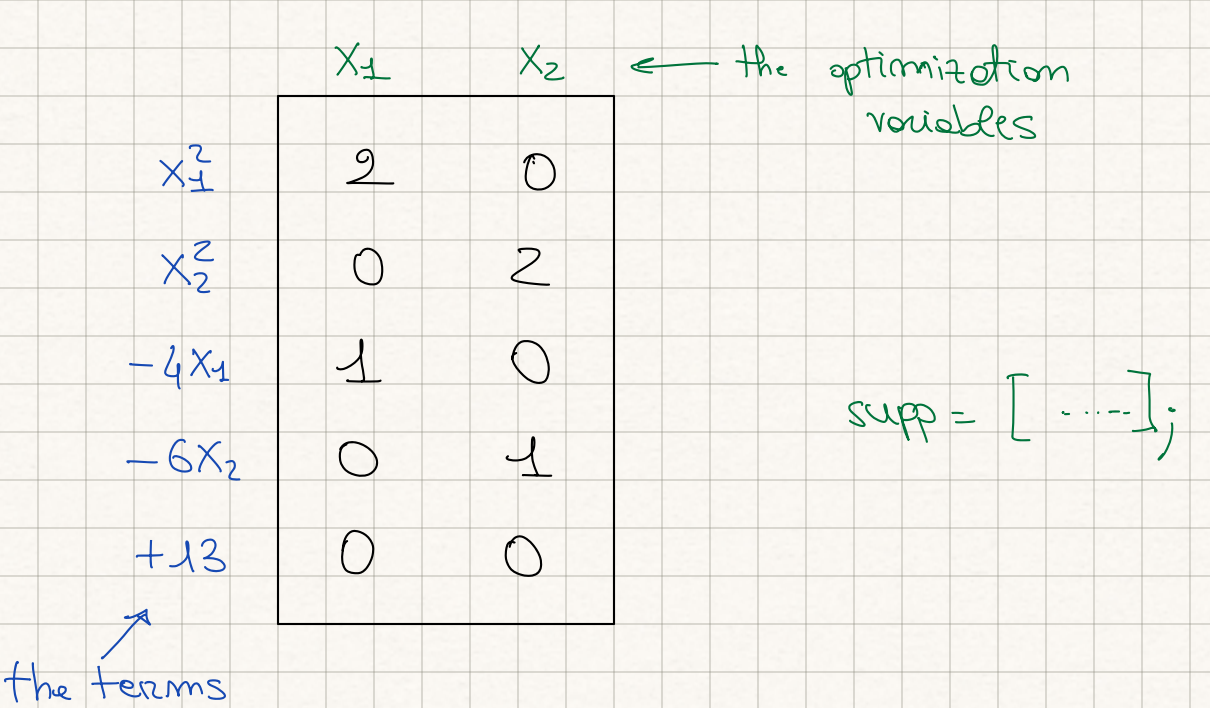
\includegraphics[width=0.75\textwidth]{images/support-matrix.png}
    \caption{The contour of the polynomial as well as the graph of the constraints}
    \label{fig:constraints}
\end{figure}

The inequality and equality constraints should be defined as cell array structures. Pay attention that:
\begin{itemize}
\item \textbf{Equality}: .typeCone = -1
\item \textbf{Inequality}: .typeCone = 1
\end{itemize}

\begin{example}[Definig the polynomila to be optimized]
\begin{lstlisting}
% equality constraint
c = 1;
ineqPolySys{c}.noTerms = 3;
ineqPolySys{c}.dimVar = 2;
ineqPolySys{c}.typeCone = -1; % equality
ineqPolySys{c}.degree = 2;
ineqPolySys{c}.supports = [1 1; 0 1; 0 0];
ineqPolySys{c}.coef = [1 -7 -10]';
% inequality constraint
c = 2;
ineqPolySys{c}.noTerms = 3;
ineqPolySys{c}.dimVar = 2;
ineqPolySys{c}.typeCone = +1; % inequality
ineqPolySys{c}.degree = 1;
ineqPolySys{c}.supports = [0 1; 1 0; 0 0];
ineqPolySys{c}.coef = [1 0.5 -1]';
\end{lstlisting}
\end{example}

After defining the lower bounds and upper bounds for the optimization variables, the \textbf{relaxation order} should be chosen. For this lab, it is recommended that one tries with relaxation orders 1, 2, 3, 4 to solve the problem.

\begin{example}[Solving the optimization problem]
\begin{lstlisting}
% lower bound
lbd = -1e10*ones(2,1);
% upper bound
ubd = +1e10*ones(2,1);

param.relaxOrder = 3;
param.POPsolver = 'interior-point';

[a,b,POP] = sparsePOP(objPoly, ineqPolySys, lbd, ubd, param);
sol_relaxed = POP.xVect;
sol_refined = POP.xVectL;

hold on; 
plot(sol_relaxed(1),sol_relaxed(2),'r*');
plot(sol_refined(1),sol_refined(2),'m*');
\end{lstlisting}
\end{example}

For relaxation order 1 and 2, it can be seen that the solution of the optimization problem does not respect the constraints. That is, the solution is not acceptable.

\begin{figure}[htbp]  % "h" for here, "t" for top, "b" for bottom, "p" for float page
    \centering
    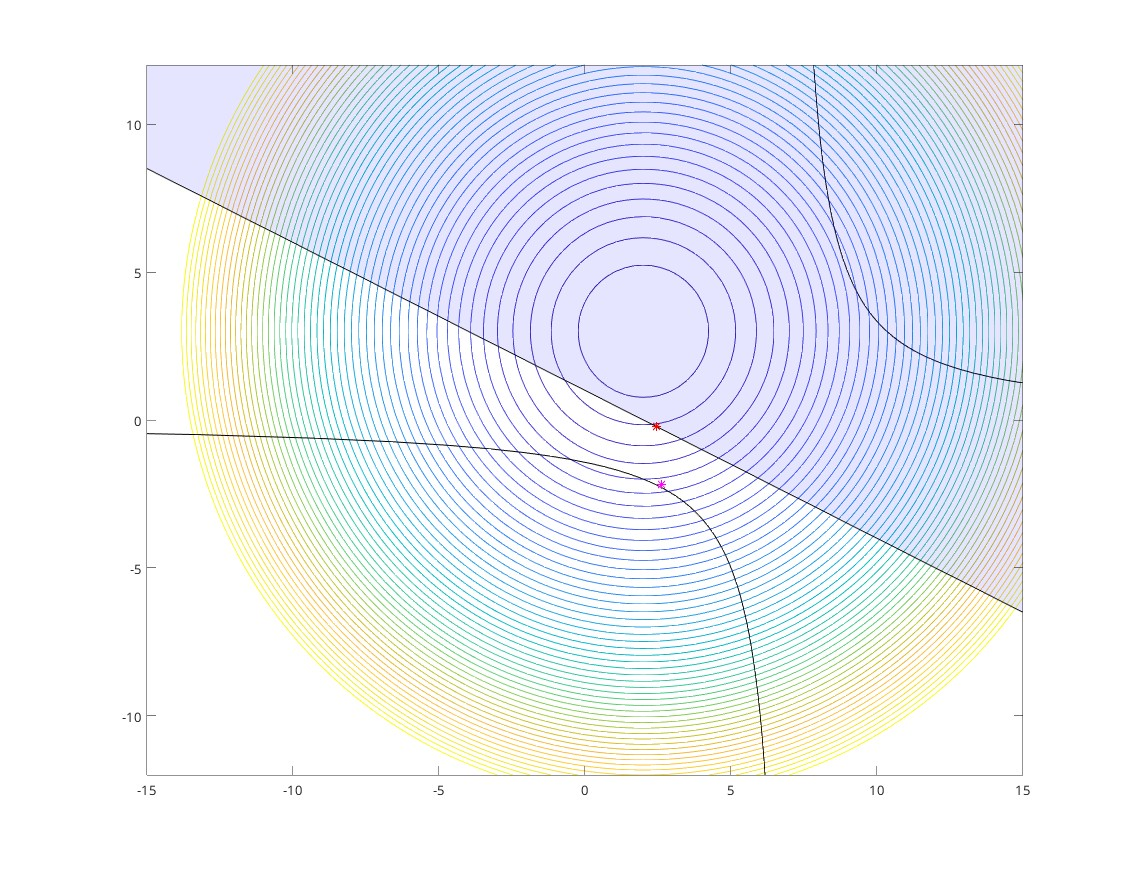
\includegraphics[width=0.75\textwidth]{images/relaxed1.jpg}
    \caption{The solution of the problem with relaxation order 1, the red star spots the relaxed solution and the other star the refined solution, which is the result of sedumi}
    \label{fig:constraints}
\end{figure}

With the relaxation order 3, the problem has an acceptable solution.


\begin{figure}[htbp]  % "h" for here, "t" for top, "b" for bottom, "p" for float page
    \centering
    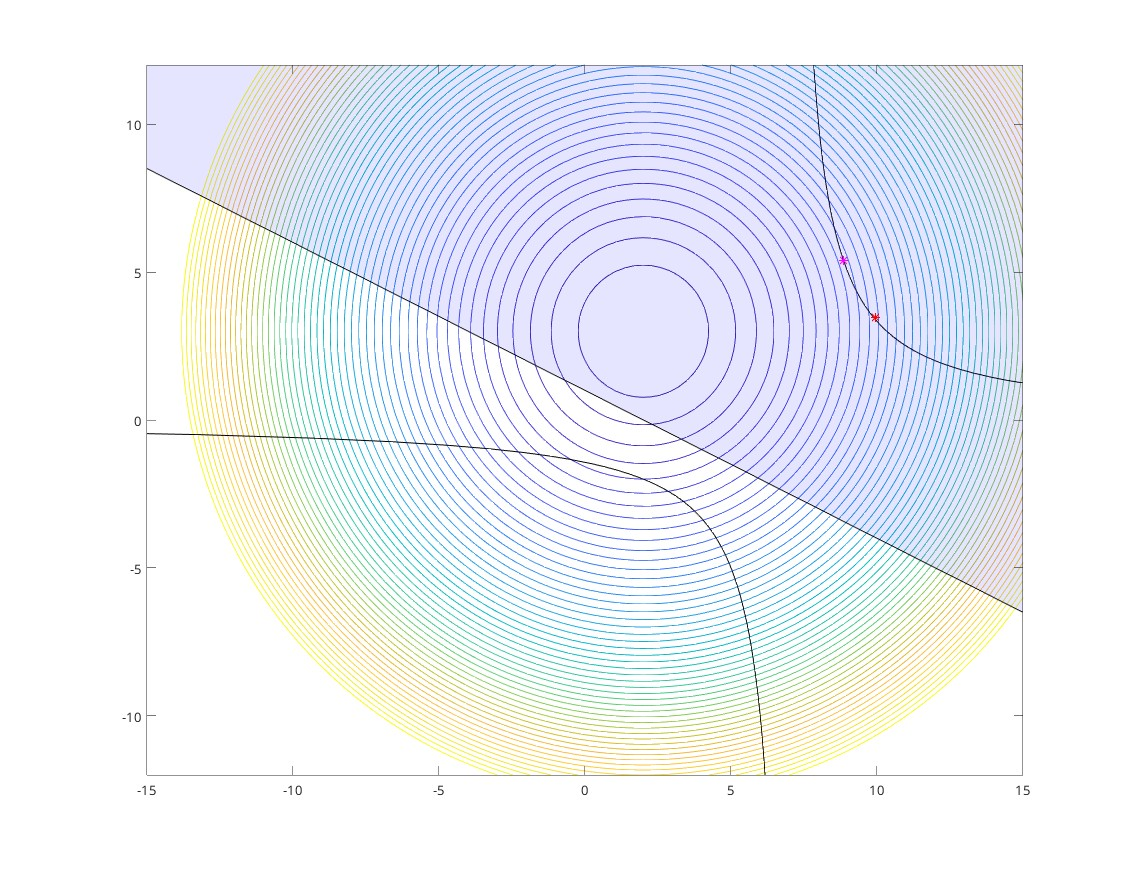
\includegraphics[width=0.75\textwidth]{images/relax3.jpg}
    \caption{The solution of the problem with relaxation order 3}
    \label{fig:constraints}
\end{figure}
